\documentclass[14pt, letterpaper, twoside]{book}

\usepackage[T1]{fontenc}
\usepackage[utf8]{inputenc}
\usepackage[utf8]{vietnam}
\usepackage[vietnam]{babel}

\usepackage[unicode]{hyperref}
\usepackage{amsmath}
\usepackage{amssymb}
\usepackage{eucal}
\usepackage{mathtools}

\usepackage{listings}
\lstset{
basicstyle=\ttfamily,
columns=fullflexible,
frame=none,
breaklines=true,
postbreak=\mbox{\textcolor{red}{$\hookrightarrow$}\space},
}

\usepackage[plain]{cite}
\usepackage{natbib}

\hypersetup{
colorlinks=true,
linkcolor=blue,
filecolor=magenta,
urlcolor=cyan,
}

\title{Ghi chú của một coder}
\author{Vũ Anh}
\date{Tháng 01 năm 2018}
\usepackage{index}



\begin{document}

  \makeindex
  \maketitle

  \tableofcontents

  \part{Lập trình}

\chapter{Python}


\section{Cơ bản}

\textbf{Vấn đề với mảng}

\begin{item}
  \item Random Sampling \footnote{tham khảo [pytorch](http://pytorch.org/docs/master/torch.html?highlight=randn#torch.randn), [numpy](https://docs.scipy.org/doc/numpy-1.13.0/reference/routines.random.html))} - sinh ra một mảng ngẫu nhiên trong khoảng (0, 1), mảng ngẫu nhiên số nguyên trong khoảng (x, y), mảng ngẫu nhiên là permutation của số từ 1 đến n
\end{item}

\section{Quản lý gói với Anaconda}

\noindent Cài đặt package tại một branch của một project trên github

\begin{lstlisting}[language=bash]
  $ pip install git+https://github.com/tangentlabs/django-oscar-paypal.git@issue/34/oscar-0.6#egg=django-oscar-paypal
\end{lstlisting}

\noindent Trích xuất danh sách package

\begin{lstlisting}[language=bash]
 $ pip freeze > requirements.txt
\end{lstlisting}

\noindent \textbf{Chạy ipython trong environment anaconda}

\noindent Chạy đống lệnh này

\begin{lstlisting}[language=bash]
  conda install nb_conda
  source activate my_env
  python -m IPython kernelspec install-self --user
  ipython notebook
\end{lstlisting}

\noindent \textbf{Interactive programming với ipython}

\noindent Trích xuất ipython ra slide (không hiểu sao default `--to slides` không work nữa, lại phải thêm tham số `--reveal-prefix` [^1]

\begin{lstlisting}[language=bash]
jupyter nbconvert "file.ipynb"
  --to slides
  --reveal-prefix "https://cdnjs.cloudflare.com/ajax/libs/reveal.js/3.1.0"
\end{lstlisting}

**Tham khảo thêm**

* https://stackoverflow.com/questions/37085665/in-which-conda-environment-is-jupyter-executing
* https://github.com/jupyter/notebook/issues/541#issuecomment-146387578
* https://stackoverflow.com/a/20101940/772391

\noindent \textbf{python 3.4 hay 3.5}

Có lẽ 3.5 là lựa chọn tốt hơn (phải có của tensorflow, pytorch, hỗ trợ mock)

### Quản lý môi trường phát triển với conda

Chạy lệnh `remove` để xóa một môi trường

\begin{lstlisting}[language=bash]
conda remove --name flowers --all
\end{lstlisting}

\section{Test với python}

\textbf{Sử dụng những loại test nào?}

Hiện tại mình đang viết unittest với default class của python là Unittest. Thực ra toàn sử dụng `assertEqual` là chính!

Ngoài ra mình cũng đang sử dụng tox để chạy test trên nhiều phiên bản python (python 2.7, 3.5). Điều hay của tox là mình có thể thiết kế toàn bộ cài đặt project và các dependencies package trong file `tox.ini`

\textbf{Chạy test trên nhiều phiên bản python với tox}

Pycharm hỗ trợ debug tox (quá tuyệt!), chỉ với thao tác đơn giản là nhấn chuột phải vào file tox.ini của project.

\section{Xây dựng docs với readthedocs và sphinx}

\noindent \textbf{20/12/2017}: Tự nhiên hôm nay tất cả các class có khai báo kế thừa ở project languageflow không thể index được. Vãi thật. Làm thằng đệ không biết đâu mà build model.

Thử build lại chục lần, thay đổi file conf.py và package\_reference.rst chán chê không được. Giả thiết đầu tiên là do hai nguyên nhân (1) docstring ghi sai, (2) nội dung trong package\_reference.rst bị sai. Sửa chán chê cũng vẫn thể, thử checkout các commit của git. Không hoạt động!

Mất khoảng vài tiếng mới để ý thằng readthedocs có phần log cho từng build một. Lần mò vào build gần nhất và build (mình nhớ là) thành công cách đây 2 ngày

\noindent Log build gần nhất

\begin{lstlisting}[language=bash]
Running Sphinx v1.6.5
making output directory...
loading translations [en]... done
loading intersphinx inventory from https://docs.python.org/objects.inv...
intersphinx inventory has moved: https://docs.python.org/objects.inv -> https://docs.python.org/2/objects.inv
loading intersphinx inventory from http://docs.scipy.org/doc/numpy/objects.inv...
intersphinx inventory has moved: http://docs.scipy.org/doc/numpy/objects.inv -> https://docs.scipy.org/doc/numpy/objects.inv
building [mo]: targets for 0 po files that are out of date
building [readthedocsdirhtml]: targets for 8 source files that are out of date
updating environment: 8 added, 0 changed, 0 removed
reading sources... [ 12%] authors
reading sources... [ 25%] contributing
reading sources... [ 37%] history
reading sources... [ 50%] index
reading sources... [ 62%] installation
reading sources... [ 75%] package_reference
reading sources... [ 87%] readme
reading sources... [100%] usage

looking for now-outdated files... none found
pickling environment... done
checking consistency... done
preparing documents... done
writing output... [ 12%] authors
writing output... [ 25%] contributing
writing output... [ 37%] history
writing output... [ 50%] index
writing output... [ 62%] installation
writing output... [ 75%] package_reference
writing output... [ 87%] readme
writing output... [100%] usage
\end{lstlisting}

Log build hồi trước

\begin{lstlisting}[language=bash]
Running Sphinx v1.5.6
making output directory...
loading translations [en]... done
loading intersphinx inventory from https://docs.python.org/objects.inv...
intersphinx inventory has moved: https://docs.python.org/objects.inv -> https://docs.python.org/2/objects.inv
loading intersphinx inventory from http://docs.scipy.org/doc/numpy/objects.inv...
intersphinx inventory has moved: http://docs.scipy.org/doc/numpy/objects.inv -> https://docs.scipy.org/doc/numpy/objects.inv
building [mo]: targets for 0 po files that are out of date
building [readthedocs]: targets for 8 source files that are out of date
updating environment: 8 added, 0 changed, 0 removed
reading sources... [ 12%] authors
reading sources... [ 25%] contributing
reading sources... [ 37%] history
reading sources... [ 50%] index
reading sources... [ 62%] installation
reading sources... [ 75%] package_reference
reading sources... [ 87%] readme
reading sources... [100%] usage

/home/docs/checkouts/readthedocs.org/user_builds/languageflow/checkouts/develop/languageflow/transformer/count.py:docstring of languageflow.transformer.count.CountVectorizer:106: WARNING: Definition list ends without a blank line; unexpected unindent.
/home/docs/checkouts/readthedocs.org/user_builds/languageflow/checkouts/develop/languageflow/transformer/tfidf.py:docstring of languageflow.transformer.tfidf.TfidfVectorizer:113: WARNING: Definition list ends without a blank line; unexpected unindent.
../README.rst:7: WARNING: nonlocal image URI found: https://img.shields.io/badge/latest-1.1.6-brightgreen.svg
looking for now-outdated files... none found
pickling environment... done
checking consistency... done
preparing documents... done
writing output... [ 12%] authors
writing output... [ 25%] contributing
writing output... [ 37%] history
writing output... [ 50%] index
writing output... [ 62%] installation
writing output... [ 75%] package_reference
writing output... [ 87%] readme
writing output... [100%] usage
\end{lstlisting}

Đập vào mắt là sự khác biệt giữa documentation type

Lỗi

\begin{lstlisting}[language=bash]
building [readthedocsdirhtml]: targets for 8 source files that are out of date
\end{lstlisting}

Chạy

\begin{lstlisting}[language=bash]
building [readthedocs]: targets for 8 source files that are out of date
\end{lstlisting}

Hí ha hí hửng. Chắc trong cơn bất loạn sửa lại settings đây mà. Sửa lại nó trong phần Settings (Admin &gt; Settings &gt; Documentation type)

![](https://magizbox.files.wordpress.com/2017/10/screenshot-from-2017-12-20-09-54-23.png)

Khi chạy nó đã cho ra log đúng

\begin{lstlisting}[language=bash]
building [readthedocsdirhtml]: targets for 8 source files that are out of date
\end{lstlisting}

Nhưng vẫn lỗi. Vãi!!! Sau khoảng 20 phút tiếp tục bấn loạn, chửi bới readthedocs các kiểu. Thì để ý dòng này

Lỗi

\begin{lstlisting}[language=bash]
Running Sphinx v1.6.5
\end{lstlisting}


Chạy

\begin{lstlisting}[language=bash]
Running Sphinx v1.5.6
\end{lstlisting}

Ngay dòng đầu tiên mà không để ý, ngu thật. Aha, Hóa ra là thằng readthedocs nó tự động update phiên bản sphinx lên 1.6.5. Mình là mình chúa ghét thay đổi phiên bản (code đã mệt rồi, lại còn phải tương thích với nhiều phiên bản nữa thì ăn c** à). Đầu tiên search với Pycharm thấy dòng này trong `conf.py`

\begin{lstlisting}[language=bash]
# If your documentation needs a minimal Sphinx version, state it here.
# needs_sphinx = '1.0'
\end{lstlisting}

Đổi thành

\begin{lstlisting}[language=bash]
# If your documentation needs a minimal Sphinx version, state it here.
needs_sphinx = '1.5.6'
\end{lstlisting}

Vẫn vậy (holy sh*t). Thử sâu một tẹo (thực sự là rất nhiều tẹo). Thấy cái này trong trang Settings

![](https://magizbox.files.wordpress.com/2017/10/screenshot-from-2017-12-20-10-01-39.png)

Ờ há. Thằng đần này cho phép trỏ đường dẫn tới một file trong project để cấu hình dependency. Haha.
Tạo thêm một file `requirements` trong thư mục `docs` với nội dung

\begin{lstlisting}
sphinx==1.5.6
\end{lstlisting}


Sau đó cấu hình nó trên giao diện web của readthedocs

![](https://magizbox.files.wordpress.com/2017/10/screenshot-from-2017-12-20-10-04-49.png)

Build thử. Build thử thôi. Cảm giác đúng lắm rồi đấy. Và... nó chạy. Ahihi

![](https://magizbox.files.wordpress.com/2017/10/screenshot-from-2017-12-20-10-06-32.png)

\textbf{Kinh nghiệm}

* Khi không biết làm gì, hãy làm 3 việc. Đọc LOG. Phân tích LOG. Và cố gắng để LOG thay đổi theo ý mình.

PS: Trong quá trình này, cũng không thèm build thằng PDF với Epub nữa. Tiết kiệm được bao nhiêu thời gian.

\section{Pycharm Pycharm}

01/2018: Pycharm là trình duyệt ưa thích của mình trong suốt 3 năm vừa rồi.

Hôm nay tự nhiên lại gặp lỗi không tự nhận unittest, không resolve được package import bởi relative path. Vụ không tự nhận unittest sửa bằng cách xóa file .idea là xong. Còn vụ không resolve được package import bởi relative path thì vẫn chịu rồi. Nhìn code cứ đỏ lòm khó chịu thật.

\section{Vì sao lại code python?}

\textbf{01/11/2017}
Thích python vì nó quá đơn giản (và quá đẹp).

[^1]: https://github.com/jupyter/nbconvert/issues/91#issuecomment-283736634
  \chapter{Xác suất}

Phần này có thêm khảo \cite{Goodfellow-et-al-2016} và giáo trình xác suất thống kê của thạc sỹ Trần Thiện Khải, đại học Trà Vinh  \footnote{\href{http://www.ctec.tvu.edu.vn/ttkhai/xacsuatthongke_dh.htm}{http://www.ctec.tvu.edu.vn/ttkhai/xacsuatthongke\_dh.htm}}

\section{Các hàm phân phối thông dụng}

\textbf{17/01/2018} Lòng vòng thế nào hôm nay lại tìm được của bạn Đỗ Minh Hải \footnote{\href{https://dominhhai.github.io/vi/2017/10/prob-com-var}{https://dominhhai.github.io/vi/2017/10/prob-com-var}}, rất hay

\subsection{Biến rời rạc}

\subsubsection{Phân phối đều - Discrete Uniform distribution}

Là phân phối mà xác suất xuất hiện của các sự kiện là như nhau.
\newline
Biến ngẫu nhiên $X$ tuân theo phân phối đều rời rạc
$$X \sim \mathcal{U} (a, b)$$
với tham số $a, b \in \mathbb Z; a < b$ là khoảng giá trị của $X$, đặt $n = b-a+1$
\newline
Ta sẽ có:
\newline
\begin{tabular}{ | l | l | }
  \hline
  Định nghĩa & Giá trị \\
  \hline
  PMF & $p(x)$ | $\dfrac{1}{n}, \forall x \in [a,b]$ \\
  \hline
  CDF - $F(x;a,b)$ & $\dfrac{x-a+1}{n}, \forall x \in [a,b]$ \\
  \hline
  Kỳ vọng - $E[X]$ & $\dfrac{a+b}{2}$ \\
  \hline
  Phương sai - $Var(X)$ & $\dfrac{n^2-1}{12}$ \\
  \hline
\end{tabular}
\newline
Ví dụ: Lịch chạy của xe buýt tại một trạm xe buýt như sau: chiếc xe buýt đầu tiên trong ngày sẽ khởi hành từ trạm này vào lúc 7 giờ, cứ sau mỗi 15 phút sẽ có một xe khác đến trạm. Giả sử một hành khách đến trạm trong khoảng thời gian từ 7 giờ đến 7 giờ 30. Tìm xác suất để hành khách này chờ:

a) Ít hơn 5 phút.

b) Ít nhất 12 phút.

\textbf{Giải}

Gọi X là số phút sau 7 giờ mà hành khách đến trạm.

Ta có: $X \sim R[0;30]$.

a) Hành khách sẽ chờ ít hơn 5 phút nếu đến trạm giữa 7 giờ 10 và 7 giờ 15 hoặc giữa 7 giờ 25 và 7 giờ 30. Do đó xác suất cần tìm là:

$$P(0<X<15) + P(25<X<30)=\frac{5}{30} + \frac{5}{30}=\frac{1}{3}$$

b) Hành khách chờ ít nhất 12 phút nếu đến trạm giữa 7 giờ và 7 giờ 3 phút hoặc giữa 7 giờ 15 phút và 7 giờ 18 phút. Xác suất cần tìm là:

$$P(0<X<3) + P(15<X<18)=\frac{3}{30} + \frac{3}{30}=\frac{1}{5}$$

\subsubsection{Phân phối Béc-nu-li - Bernoulli distribution}

Như đã đề cập về phép thử Béc-nu-li rằng mọi phép thử của nó chỉ cho 2 kết quả duy nhất là $A$ với xác suất $p$ và $\bar A$ với xác suất $q=1-p$
Biến ngẫu nhiên $X$ tuân theo phân phối Béc-nu-li
$$X \sim B(p)$$
với tham số $p \in \mathbb{R}, 0 \leq p \leq 1$ là xác suất xuất hiện của $A$ tại mỗi phép thử
\newline
\begin{tabular}{ | l | l | l | }
  \hline
  Định nghĩa & & Giá trị \\
  \hline
  PMF & p(x) & $p(x)$ | $p^x (1-p)^{1-x}, x \in \{0, 1\} $ \\
  \hline
  CDF & $F(x;p)$  &
  \begin{cases}
    0 & \text{for } x < 0 \\
    1-p & \text{for } 0 \leq x < 1 \\
    1 & \text{for } x \geq 1
  \end{cases} \\
  \hline
  Kỳ vọng & $E[X]$ & $p$ \\
  \hline
  Phương sai & $Var(X)$ & $p(1-p)$ \\
  \hline
\end{tabular}
\newline

\textbf{Ví dụ}

Tham khảo thêm các thuật toán khác tại \cite{hai_2018}
  \part{Khoa học máy tính}

\chapter{Hệ điều hành}

\textbf{Những phần mềm không thể thiếu}

\begin{itemize}
  \item Adblock extension
  \item Trình duyệt Google Chrome (với các extensions Scihub, Mendeley Desktop, Adblock)
  \item Terminal (Oh-my-zsh)
  \item IDE Pycharm để code python
  \item Quản lý phiên bản code Git
  \item Bộ gõ ibus-unikey trong Ubuntu hoặc unikey (Windows) (Ctrl-Space để chuyển đổi ngôn ngữ)
  \item CUDA (lập trình trên GPU)
\end{itemize}

\textbf{Xem thông tin hệ thống}

Phiên bản `ubuntu 16.04`

\begin{lstlisting}
sudo apt-get install sysstat
\end{lstlisting}


Xem hoạt động (\%) của các core cpu

\begin{lstlisting}
mpstat -A
\end{lstlisting}


CPU của mình có bao nhiều core, bao nhiêu siblibngs

\begin{lstlisting}
cat /proc/cpuinfo

processor       : 23
vendor_id       : GenuineIntel
cpu family      : 6
model           : 62
model name      : Intel(R) Xeon(R) CPU E5-2430 v2 @ 2.50GHz
stepping        : 4
microcode       : 0x428
cpu MHz         : 1599.707
cache size      : 15360 KB
physical id     : 1
siblings        : 12
core id         : 5
cpu cores       : 6
apicid          : 43
initial apicid  : 43
fpu             : yes
fpu_exception   : yes
cpuid level     : 13
wp              : yes
flags           : fpu vme de pse tsc msr pae mce cx8 apic sep mtrr pge mca cmov pat pse36 clflush dts acpi mmx fxsr sse sse2 ss ht tm pbe syscall nx pdpe1gb rdtscp lm constant_tsc arch_perfmon pebs bts rep_good nopl xtopology nonstop_tsc aperfmperf eagerfpu pni pclmulqdq dtes64 monitor ds_cpl vmx smx est tm2 ssse3 cx16 xtpr pdcm pcid dca sse4_1 sse4_2 x2apic popcnt tsc_deadline_timer aes xsave avx f16c rdrand lahf_lm ida arat xsaveopt pln pts dtherm tpr_shadow vnmi flexpriority ept vpid fsgsbase smep erms
bogomips        : 5005.20
clflush size    : 64
cache_alignment : 64
address sizes   : 46 bits physical, 48 bits virtual
power management:
\end{lstlisting}

Kết quả cho thấy cpu của 6 core và 12 siblings

\textbf{Xem chương trình nào tốn ram}


\begin{lstlisting}
ps aux | awk '{print $2, $4, $11}' | sort -k2rn | head -n 20
\end{lstlisting}

\href{https://www.garron.me/en/go2linux/how-find-which-process-eating-ram-memory-linux.html}{https://www.garron.me/en/go2linux/how-find-which-process-eating-ram-memory-linux.html}


\chapter{Ubuntu}

\diary{27/12/2017: Lại dính lỗi không thể login. Lần này thì lại phải xóa bạn KDE đi. Kể cũng hơn buồn. Nhưng nhất quyết phải enable được tính năng Windows Spreading (hay đại loại thế). Hóa ra khi ubuntu bị lỗi không có lancher hay toolbar là do bạn unity plugin chưa được enable. Oài. Sao người hiền lành như mình suốt ngày bị mấy lỗi vớ vẩn thế không biết.}

\diary{20/11/2017: Hôm nay đen thật, dính lỗi login loop. Fix mãi mới được. Thôi cũng kệ. Cảm giác bạn KDE này đỡ bị lỗi ibus-unikey hơn bạn GNOME. Hôm nay cũng đổi bạn zsh theme. Chọn mãi chẳng được bạn nào ổn ổn, nhưng không thể chịu được kiểu suggest lỗi nữa rồi. Đôi khi thấy default vẫn là tốt nhất.}

\diary{21/11/2017: Sau một ngày trải nghiệm KDE, cảm giác giao diện mượt hơn GNOME. Khi overview windows với nhiều màn hình tốt và trực quan hơn. Đặc biệt là không bị lỗi ibus nữa. Đổi terminal cũng cảm giác ổn ổn. Không bị lỗi suggest nữa.}

\textbf{Chuyện terminal}

Terminal là một câu chuyện muôn thưở của bất kì ông coder nào thích customize, đẹp, tiện (và bug kinh hoàng). Hiện tại mình đang thấy combo này khá ổn Terminal (Ubuntu) (Color: Black on white, Build-in schemes: Tango) + zsh + oh-my-zsh (fishy-custom theme). Những features hay ho

\begin{itemize}
  \item Làm việc tốt trên cả Terminal (white background) và embedded terminal của Pycharm (black background)
  \item Hiển thị folder dạng ngắn (chỉ ký tự đầu tiên)
  \item Hiển thị brach của git ở bên phải
\end{itemize}


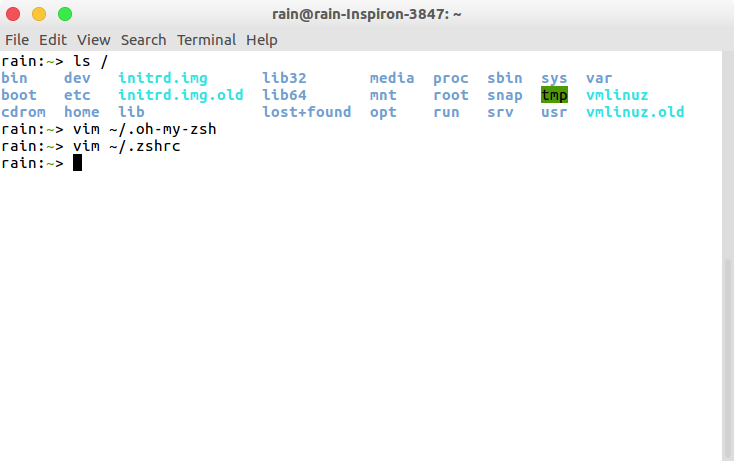
\includegraphics[width=10cm]{images/computer_science/ubuntu/terminal.png}

\textbf{Chuyện bộ gõ}

Làm sao để khởi động lại ibus, thỉnh thoảng lại chết bất đắc kì tử

\begin{lstlisting}
ibus-daemon &
ibus restart
\end{lstlisting}

\textbf{Chuyện lỗi login loop}

Phiên bản: `ubuntu 16.04`



\href{https://askubuntu.com/questions/389903/ibus-doesnt-seem-to-restart}{https://askubuntu.com/questions/389903/ibus-doesnt-seem-to-restart}

\textbf{Hot Corner và Workspace}

Cần cài đặt ngay \textbf{gnome-tweak-tool}

\begin{lstlisting}
sudo apt install gnome-tweak-tool
\end{lstlisting}

Cài đặt hot corner với

\href{https://askubuntu.com/questions/975348/how-to-get-all-hot-corner-in-ubuntu-17-10}{https://askubuntu.com/questions/975348/how-to-get-all-hot-corner-in-ubuntu-17-10}

Cài đặt Workspace
  \chapter{Học máy}

View online \href{http://magizbox.com/training/machinelearning/site/}{http://magizbox.com/training/machinelearning/site/}

\begin{itemize}
  \item Vấn đề với HMM và CRF?
  \item Học MLE và MAP?
\end{itemize}



Machine learning is a branch of science that deals with programming the systems in such a way that they automatically learn and improve with experience. Here, learning means recognizing and understanding the input data and making wise decisions based on the supplied data.

We can think of machine learning as approach to automate tasks like predictions or modelling. For example, consider an email spam filter system, instead of having programmers manually looking at the emails and coming up with spam rules. We can use a machine learning algorithm and feed it input data (emails) and it will automatically discover rules that are powerful enough to distinguish spam emails.

Machine learning is used in many application nowadays like spam detection in emails or movie recommendation systems that tells you movies that you might like based on your viewing history. The nice and powerful thing about machine learning is: It learns when it gets more data and hence it gets more and more powerful the more data we give them.

**Có bao nhiêu thuật toán Machine Learning?**

Có rất nhiều thuật toán Machine Learning, bài viết [Điểm qua các thuật toán Machine Learning hiện đại](https://ongxuanhong.wordpress.com/2015/10/22/diem-qua-cac-thuat-toan-machine-learning-hien-dai/) của Ông Xuân Hồng tổng hợp khá nhiều thuật toán. Theo đó, các thuật toán Machine Learning được chia thành các nhánh lớn như `regression`, `bayesian`, `regularization`, `decision tree`, `instance based`, `dimesionality reduction`, `clustering`, `deep learning`, `neural networks`, `associated rule`, `ensemble`... Ngoài ra thì còn có các cheatsheet của [sklearn](http://scikit-learn.org/stable/tutorial/machine_learning_map/index.html).

Việc biết nhiều thuật toán cũng giống như ra đường mà có nhiều lựa chọn về xe cộ. Tuy nhiên, quan trọng là có task để làm, sau đó thì cập nhật SOTA của task đó để biết các công cụ mới.

**Xây dựng model cần chú ý điều gì?**

Khi xây dựng một model cần chú ý đến vấn đề tối ưu hóa tham số (có thể sử dụng [GridSearchCV](sklearn.model_selection.GridSearchCV))

Bài phát biểu này có vẻ cũng rất hữu ích [PYCON UK 2017: Machine learning libraries you'd wish you'd known about](https://www.youtube.com/watch?v=nDF7_8FOhpI). Có đề cập đến

* [DistrictDataLabs/yellowbrick](https://github.com/DistrictDataLabs/yellowbrick) (giúp visualize model được train bởi sklearn)
* [marcotcr/lime](https://github.com/marcotcr/lime) (giúp inspect classifier)
* [TeamHG-Memex/eli5](https://github.com/TeamHG-Memex/eli5) (cũng giúp inspect classifier, hỗ trợ nhiều model như xgboost, crfsuite, đặc biệt có TextExplainer sử dụng thuật toán từ eli5)
* [rhiever/tpot](https://github.com/rhiever/tpot) (giúp tối ưu hóa pipeline)
* [dask/dask](https://github.com/dask/dask) (tính toán song song và lập lịch)

Ghi chú về các thuật toán trong xử lý ngôn ngữ tự nhiên tại [underthesea.flow/wiki](https://github.com/magizbox/underthesea.flow/wiki/Develop)

Framework để train, test hiện tại vẫn rất thoải mái sklearn. tensorboard cung cấp phần log cũng khá hay.

[Câu trả lời hay](https://www.quora.com/What-are-the-most-important-machine-learning-techniques-to-master-at-this-time/answer/Sean-McClure-3?srid=5O2u) cho câu hỏi [Những kỹ thuật machine learning nào quan trọng nhất để master?](https://www.quora.com/What-are-the-most-important-machine-learning-techniques-to-master-at-this-time), đặc biệt là dẫn đến bài [The State of ML and Data Science 2017](https://www.kaggle.com/surveys/2017) của Kaggle.

**Tài liệu học PGM**

[Playlist youtube](https://www.youtube.com/watch?v=WPSQfOkb1M8&amp;list=PL50E6E80E8525B59C) khóa học Probabilistic Graphical Models của cô Daphne Koller. Ngoài ra còn có một [tutorial](http://mensxmachina.org/files/software/demos/bayesnetdemo.html) dở hơi ở đâu về tạo Bayesian network

**[Chưa biết] Tại sao Logistic Regression lại là Linear Model?**

Trong quyển Deep Learning, chương 6, trang 165, tác giả có viết

```
Linear models, such as logistic regression and linear
regression, are appealing because they can be fit
efficiently and reliably, either in closed form or
with convex optimization
```

Mình tự hỏi tại sao logistic regression lại là linear, trong khi nó có sử dụng hàm logit (nonlinear)? Tìm hiểu hóa ra cũng có bạn hỏi giống mình trên [stats.stackexchange.com](https://stats.stackexchange.com/questions/93569/why-is-logistic-regression-a-linear-classifier). Ngoài câu trả lời trên stats.stackexchange, đọc một số cái khác [Generalized Linear Models, SPSS Statistics 22.0.0](https://www.ibm.com/support/knowledgecenter/en/SSLVMB_22.0.0/com.ibm.spss.statistics.help/spss/advanced/idh_idd_genlin_typeofmodel.htm)
và [6.1 - Introduction to Generalized Linear Models, Analysis of Discrete Data, Pennsylvania State University](https://onlinecourses.science.psu.edu/stat504/node/216) cũng vẫn chưa hiểu lắm.

Hiện tại chỉ hiểu là các lớp model này chỉ có thể hoạt động trên các tập linear separable, có lẽ do việc map input x, luôn có một liên kết linear $latex wx$, trước khi đưa vào hàm non-linear.

**Các tập dữ liệu thú vị**

*Iris dataset*: dữ liệu về hoa iris

Là một ví dụ cho bài toán phân loại

*Weather problem*: dữ liệu thời tiết. Có thể tìm được ở trong quyển Data Mining: Practical Machine Learning Tools and Techniques

Là một ví dụ cho bài toán cây quyết định

## Deep Learning

**Tài liệu Deep Learning**

Lang thang thế nào lại thấy trang này [My Reading List for Deep Learning!](https://www.microsoft.com/en-us/research/wp-content/uploads/2017/02/DL_Reading_List.pdf) của một anh ở Microsoft. Trong đó, (đương nhiên) có Deep Learning của thánh Yoshua Bengio, có một vụ hay nữa là bài review "Deep Learning" của mấy thánh Yann Lecun, Yoshua Bengio, Geoffrey Hinton trên tạp chí Nature. Ngoài ra còn có nhiều tài liệu hữu ích khác.

### Các layer trong deep learning [^2]

#### Sparse Layers

[**nn.Embedding**](http://pytorch.org/docs/master/nn.html#embedding) ([hướng dẫn](http://pytorch.org/tutorials/beginner/nlp/word_embeddings_tutorial.html))
★ grep code: [Shawn1993/cnn-text-classification-pytorch](https://github.com/Shawn1993/cnn-text-classification-pytorch/blob/master/model.py#L18)
Đóng vai trò như một lookup table, map một word với dense vector tương ứng

#### Convolution Layers

[**nn.Conv1d**](http://pytorch.org/docs/master/nn.html#conv1d), [**nn.Conv2d**](http://pytorch.org/docs/master/nn.html#conv2d), [**nn.Conv3d**](http://pytorch.org/docs/master/nn.html#conv3d) [^1]
★ grep code: [Shawn1993/cnn-text-classification-pytorch](https://github.com/Shawn1993/cnn-text-classification-pytorch/blob/master/model.py#L20-L24), [galsang/CNN-sentence-classification-pytorch](https://github.com/galsang/CNN-sentence-classification-pytorch/blob/master/model.py#L36-L38)

Các tham số trong Convolution Layer

* `kernel_size` (hay là filter size)

Đối với NLP, kernel_size thường bằng region_size * word_dim (đối với conv1d) hay (region_size, word_dim) đối với conv2d

<small>Quá trình tạo feature map đối với region size bằng 2</small>
![](https://media.giphy.com/media/l2QE2y1UQP7vIgiti/giphy.gif)

* `in_channels`, `out_channels` (là số lượng `feature maps`)

Kênh (channels) là các cách nhìn (view) khác nhau đối với dữ liệu. Ví dụ, trong ảnh thường có 3 kênh RGB (red, green, blue), có thể áp dụng convolution giữa các kênh. Với văn bản cũng có thể có các kênh khác nhau, như khi có các kênh sử dụng các word embedding khác nhau (word2vec, GloVe), hoặc cùng một câu nhưng biểu diễn ở các ngôn ngữ khác nhau.

* `stride`

Định nghĩa bước nhảy của filter.

![](http://d3kbpzbmcynnmx.cloudfront.net/wp-content/uploads/2015/11/Screen-Shot-2015-11-05-at-10.18.08-AM-1024x251.png)

Hình minh họa sự khác biệt giữa các feature map đối với stride=1 và stride=2. Feature map đối với stride = 1 có kích thước là 5, feature map đối với stride = 3 có kích thước là 3. Stride càng lớn thì kích thước của feature map càng nhỏ.

Trong bài báo của Kim 2014, `stride = 1` đối với `nn.conv2d` và `stride = word_dim` đối với `nn.conv1d`

Toàn bộ tham số của mạng CNN trong bài báo Kim 2014,

![](http://d3kbpzbmcynnmx.cloudfront.net/wp-content/uploads/2015/11/Screen-Shot-2015-11-06-at-8.03.47-AM.png)

| Description | Values |
|---------------------|-----------------|
| input word vectors | Google word2vec |
| filter region size | (3, 4, 5)       |
| feature maps | 100 |
| activation function | ReLU |
| pooling | 1-max pooling |
| dropout rate | 0.5 |
| $latex l&amp;s=2$2 norm constraint | 3 |

Đọc thêm:

* [Lecture 13: Convolutional Neural Networks (for NLP). CS224n-2017](http://web.stanford.edu/class/cs224n/lectures/cs224n-2017-lecture13-CNNs.pdf)
* [DeepNLP-models-Pytorch - 8. Convolutional Neural Networks](https://nbviewer.jupyter.org/github/DSKSD/DeepNLP-models-Pytorch/blob/master/notebooks/08.CNN-for-Text-Classification.ipynb)
* [A Sensitivity Analysis of (and Practitioners’ Guide to) Convolutional Neural Networks for Sentence Classification. Zhang 2015](https://arxiv.org/pdf/1510.03820.pdf)

**BTS**

22/11/2017 - Phải nói quyển này hơi nặng so với mình. Nhưng thôi cứ cố gắng vậy.
24/11/2017 - Từ hôm nay, mỗi ngày sẽ ghi chú một phần (rất rất nhỏ) về Deep Learning [tại đây](https://docs.google.com/document/d/1KxDrw5s6uYHNLda7t0rhp0RM_TlUGxydQ-Qi1JOPFr8/edit?usp=sharing)

[^1]: [Understanding Convolutional Neural Networks for NLP](http://www.wildml.com/2015/11/understanding-convolutional-neural-networks-for-nlp)
[^2]: [http://pytorch.org/docs/master/nn.html](http://pytorch.org/docs/master/nn.html)

\section{Machine Learning Process}

The good life is a process, not a state of being. It is a direction not a destination.

Carl Rogers


I searched a framework fit for every data mining task, I found a good one from an article of Oracle.

And here is my summary. The data mining process has 4 steps:

Step 1. Problem Definition

This initial phase of a data mining project focuses on understanding the project objectives and requirements. Once you have specified the project from a business perspective, you can formulate it as a data mining problem and develop a preliminary implementation plan.

Step 2. Data Gathering & Preparation

The data understanding phase involves data collection and exploration. As you take a closer look at the data, you can determine how well it addresses the business problem. You might decide to remove some of the data or add additional data. This is also the time to identify data quality problems and to scan for patterns in the data.

Data Access
Data Sampling

Data Transformation

Data in the real world is dirty [3]. They are often incomplete (lacking attribute values, lacking certain attributes of interest, or containing only aggregate data), noisy (containing errors or outliers),‰ inconsistent (containing discrepancies in codes or names). Step 3. Model Building In this phase, you select and apply various modeling techniques and calibrate the parameters to optimal values. If the algorithm requires data transformations, you will need to step back to the previous phase to implement them

Create Model
Test Model

Evaluate & Interpret Model

Some important questions [2]:

Is at least one of predictors useful in predicting the response? (F-statistics)
Do all the predictors help to explain Y, or is only a subset of the predictors useful? (all subsets or best subsets)
How well does the model fit the data?
Given a set of predictor values, what response value should we predict, and how accurate is our prediction?
Step 4. Knowledge Deployment Knowledge deployment is the use of data mining within a target environment. In the deployment phase, insight and actionable information can be derived from data.
Model Apply
Custom Reports
External Applications
References
The Data Mining Process, Oracle
Trevor Hastie and Rob Tibshirani, Model Selection and Qualitative Predictors, URL:https://www.youtube.com/watch?v=3T6RXmIHbJ4
Nguyen Hung Son, Data cleaning and Data preprocessing, URL:http://www.mimuw.edu.pl/~son/datamining/DM/4-preprocess.pdf

\subsection{Problem Definition}

This initial phase of a data mining project focuses on understanding the project objectives and requirements. Once you have specified the project from a business perspective, you can formulate it as a data mining problem and develop a preliminary implementation plan.

For example, your business problem might be: "How can I sell more of my product to customers?" You might translate this into a data mining problem such as: "Which customers are most likely to purchase the product?" A model that predicts who is most likely to purchase the product must be built on data that describes the customers who have purchased the product in the past. Before building the model, you must assemble the data that is likely to contain relationships between customers who have purchased the product and customers who have not purchased the product. Customer attributes might include age, number of children, years of residence, owners/renters, and so on.

\subsection{Data Gathering}

The data understanding phase involves data collection and exploration. As you take a closer look at the data, you can determine how well it addresses the business problem. You might decide to remove some of the data or add additional data. This is also the time to identify data quality problems and to scan for patterns in the data.

The data preparation phase covers all the tasks involved in creating the case table you will use to build the model. Data preparation tasks are likely to be performed multiple times, and not in any prescribed order. Tasks include table, case, and attribute selection as well as data cleansing and transformation. For example, you might transform a DATE_OF_BIRTH column to AGE; you might insert the average income in cases where the INCOME column is null.

Additionally you might add new computed attributes in an effort to tease information closer to the surface of the data. For example, rather than using the purchase amount, you might create a new attribute: "Number of Times Amount Purchase Exceeds $500 in a 12 month time period." Customers who frequently make large purchases may also be related to customers who respond or don't respond to an offer.

Thoughtful data preparation can significantly improve the information that can be discovered through data mining.

Data Sources
Open Data

wikipedia dumps: https://dumps.wikimedia.org/other/pagecounts-raw/

\subsection{Data Preprocessing}

The quality of the data and the amount of useful information it contains affect greatly how well an algorithm can learn. Hence, it is important to preprocess the dataset before using it. The most common preprocessing steps are: removing missing values, converting categorical data into shape suitable for machine learning algorithm and feature scaling.

Missing Data
Sometimes the samples in the dataset are missing some values and we want to deal with these missing values before passing it to the machine learning algorithm. There are a number of strategies we can follow

Remove samples with missing values: This approach is by far the most convenient but we may end up removing too many samples and by that we would be losing valuable information that can help the machine learning algorithm.
Imputing missing values: Instead of removing the entire sample we use interpolation to estimate the missing values. For example, we could substitute a missing value by the mean of the entire column.
Categorical Data
In general, features can be numerical (e.g. price, length, width, etc…) or categorical (e.g. color, size, etc..). Categorical features are further split into nominal and ordinal features.

Ordinal features can be sorted and ordered. For example, size (small, medium, large), we can order these sizes large > medium > small. While nominal features do not have an order for example, color, it doesn’t make any sense to say that red is larger than blue.

Most machine learning algorithm require that you convert categorical features into numerical values. One solution would to assign each value a different number starting from zero. (e.g. small à 0 ,medium à 1 ,large à 2)

This works well for ordinal features but might cause problems with nominal features (e.g. blue à 0, white à 1, yellow à 2) because even though colors are not ordered the learning algorithm will assume that white is larger than blue and yellow is larger than white and this is not correct.

To get around this problem is to use one-hot encoding, the idea is to create a new feature for each unique value of the nominal feature.


In the above example, we converted the color feature into three new features Red, Green, Blue and we used binary values to indicate the color. For example, a sample with “Red” color is now encoded as (Red=1, Green=0, Blue=0)

Feature Scaling
Why have we do Feature Scaling?

We have to predict the house prices base on 2 features:

House sizes (feet2)
Number of bedrooms in the house
And we relized that house sizes are about 1000 times the number of bedrooms. When features differ by orders of magnitude, first performing feature scaling can make gradient descent converge much more quickly.

Perform Feature Scaling

Subtract the mean value (the average value) of each feature from the dataset.
After subtracting the mean, additionally scale (divide) the feature values by their respective "standard deviations."
Function: x′=x−x¯σx′=x−x¯σ where xx is the original feature vector, x¯x¯ is the mean of that feature vector, and σσ is its standard deviation.
Feature Scaling Function implementation in Octave

function [X_norm, mu, sigma] = featureNormalize(X)
X_norm = X;
mu = zeros(1, size(X, 2)); % storing the mean value in mu
sigma = zeros(1, size(X, 2)); % storing the standard deviation in sigma

for i = 1:length(mu),
mu(i) = mean(X(:,i));
end;

for i = 1:length(sigma),
sigma(i) = std(X(:,i));
end;

X_norm = (X .- mu)./sigma;
end
Related Reading
Introduction to Machine Learning

\subsection{Model Building}

In this phase, you select and apply various modeling techniques and calibrate the parameters to optimal values. If the algorithm requires data transformations, you will need to step back to the previous phase to implement them

Create Model
Test Model
Evaluate & Interpret Model
Some important questions

Is at least one of predictors useful in predicting the response? (F-statistics)
Do all the predictors help to explain Y, or is only a subset of the predictors useful? (all subsets or best subsets)
How well does the model fit the data?
Given a set of predictor values, what response value should we predict, and how accurate is our prediction?
Create Model
First thing first, start with simple and fast model, then you known how difficult the problem is.

One import thing is create a well pipeline for your experiments, it is very helpful in turning features, model selection, save your experiment and write reports.

Feature Selections
After train model, some model will give active features (such as CRF), it is clue for you to feature selection. If amount active features is too small compared to amount features, it is the problem. In this case the better way to enhance is try reduce amount of features and see how well this set fit data. Keep in mind the more number of features is, the complex model is, and it will make your model over fitting.
Storing the model
Number of active features: 5566 (35383)
Number of active attributes: 4343 (20722)
example after training crf model with python-crfsuite
Test Model
This phase determines how well the model fit data. See Evaluation for details.

What to do next
In an interview Andrew Ng said about building machine learning model

"I often make an analogy to building a rocket ship. A rocket ship is a giant engine together with a ton of fuel. Both need to be really big. If you have a lot of fuel and a tiny engine, you won’t get off the ground. If you have a huge engine and a tiny amount of fuel, you can lift up, but you probably won’t make it to orbit. So you need a big engine and a lot of fuel.

The reason that machine learning is really taking off now is that we finally have the tools to build the big rocket engine — that is giant computers, that’s our rocket engine. And the fuel is the data. We finally are getting the data that we need."

We need both big rocket engine and data to make our model works.

Related Reading
Inside The Mind That Built Google Brain: On Life, Creativity, And Failure, huffingtonpost.com

\subsection{Evaluation}

Training vs Test Data
We typically split the input data into learning and testing datasets. The then run the machine learning algorithm on the learning dataset to generate the prediction model. Later, we use the test dataset to evaluate our model.


It is important that the test data is separate from the one used in training otherwise we will be kind of cheating because may for example the generated model memorizes the data and hence if the test data is also part of the training data then our evaluation scores of the model will be higher than they actually are.

The data is usually split 75% training and 25% data or 2/3 training and 1/3 testing. It is important to note that: the smaller the training set the more challenging it is for the algorithm to discover the rules.

In addition, when splitting the dataset, you need to maintaining class proportions and population statistics otherwise we will have some classes that are under represented in the training dataset and over represented in the test dataset.

For example, you may have 100 sample and a total of 80 samples are labeled with Class-A and the remaining 20 instances are labeled with Class-B. you want to make sure when splitting the data that you maintain this representation.

One way to avoid this problem and to make sure that all classes are represented in both training and testing datasets is stratification. It is the process of rearranging the data as to ensure each set is a good representative of the whole. In our previous example, (80/20 samples), it is best to arrange the data such that in every set, each class comprises around 80:20 ratios of the two classes.

Cross Validation
A crucial step when building our machine learning model is to estimate its performance on that that the model hadn't seen before. We want to make sure that the model generalizes well to new unseen data.

One case, the machine learning algorithm has different parameters and we want to tune these parameters to achieve the best performance. (Note: the parameters of the machine learning algorithm are called hyperparameters). Another case, sometimes we want to try out different algorithms and choose the best performing one. Below are some of the techniques used.

Holdout Method
We simply split the data into training and testing datasets. We train the algorithm on the training dataset to generate a model. In order, to evaluate different algorithms we use the testing data to evaluate each algorithm.

However, if we reuse the same test dataset over and over again during algorithm selection, the test data has now come part of the training data. Hence, when we use the test data for the final evaluation the generated model is biased towards the test data and the performance score is optimistic.

Holdout Validation
As before, we split the data into training and testing dataset. Then, the training data is further split into training and validation sets.

The training data is used to train different models. Then the validation data is used to compute performance of each of them and we select the best one. Finally, the model is then used for the test set to evaluate performance. The next figure illustrates this idea.


However, because we use the validation set multiple times, Holdout validation is sensitive to how we partition the data and that is what K-fold cross validation tries to solve.

K-fold cross validation
Initially, we split the data into training and testing dataset. Furthermore, the training dataset is split into K chunks.

Suppose we will use 5-fold cross validation, the training data set is split into 5 chunks and the training phase will take place over 5 iterations. In each iteration we use one chunk as the validation dataset while the rest of the chunk are grouped together to form the training dataset.

This is very similar to Holdout validation except in each iteration the validation data is different and this removed the bias. Each iteration generates a score and the final score is the average score of all iteration. As before we select the best model and use the test data for the final performance evaluation.

Related Readings

Introduction to Machine Learning

\section{Types of Machine Learning}

There are three different types of machine learning: supervised, unsupervised and reinforcement learning. 4

Supervised Learning
The goal of supervised learning is to learn a model from labelled training data that allows us to make predictions about future data. For supervised machine learning to work we need to feed the algorithm two things: the input data and our knowledge about it labels).

The spam filter example mentioned earlier is a good example of supervised learning; we have a bunch of emails (data) and we know whether each email is spam or not (labels).


Supervised learning can be divided into two subcategories:

Classification: It is used to predict categories or class labels based on past observations i.e. we have discrete variable you want to distinguish into discrete categorical outcome. For example, in the email spam filter system the output is discrete "spam" or "not spam".
Regression: It is used to predict a continuous outcome. For example, to determine the price of houses and how it is affected by the number of rooms in that house. The input data is the house features (no. of rooms, location, size in square feet,) and the output is the price (the continuous outcome).
Unsupervised Learning
The goal of unsupervised learning is to discover hidden structure or patterns in unlabeled data and it can be divided into two subcategories

Clustering: It is used to organize information into meaningful clusters (subgroups) without having prior knowledge of their meaning. For example, the figure below shows how we can use clustering to organize unlabeled data into groups based on their features.


Dimensionality Reduction (Compression): It is used to reduce a higher dimension data into a lower dimension ones. To put it more clearly consider this example. A telescope has terabytes of data and not all of these data can be stored and so we can use dimensionality reduction to extract the most informative features of these data to be stored. Dimensionality reduction is also a good candidate to visualize data because if you have data in higher dimensions you can compress it to 2D or 3D to easily plot and visualize it.

Reinforcement Learning

The goal of reinforcement learning is to develop a system that improves its performance based on the interaction with a dynamic environment and there is a delayed feedback that act as a reward. i.e. reinforcement learning is learning by doing with a delayed reward. A classic example of reinforcement learning is a chess game, the computer decided a series of moves and the reward is the "win" or "lose" at the end the game.

You might think that this is similar to supervised learning where the reward is basically a label for the data but the core difference is this feedback/reward is not the truth but it is a measure of how well the action to achieving a certain goal.

Microsoft Azure Machine Learning 1


Machine Learning Cheat Sheet for scikit-learn 2


DLib C++ Library - Machine Learning Guide 3


Challenges
Very much features (> 100)
Very much data (> 1e9 items)
Text Data, Images, Videos
Training Times
Accuracy, Over Fitting
Machine learning algorithm cheat sheet for Microsoft Azure Machine Learning Studio ↩

Machine Learning Cheat Sheet (for scikit-learn) ↩

DLib C++ Library - Machine Learning Guide ↩

Introduction to Machine Learning ↩

\section{How to learn a ML Algorithm?}

1. Motivation

Each algorithm have its own motivation. It may a simple example to see how it work

2. Problem Definition

Where can we apply this algorithm? How did it work in real world applications

3. Mathematics Representation

Problem Equations, notations

We will discuss about mathematics representation of algorithm, notations we use for problem

4. Algorithm

We will discuss how to solve this mathematics problems

5. Examples

We will apply algorithm with a few examples (1-2 dimension is highly recommended, because we will plot these data and model easily)

In this section, we can see how well (bad) algorithm works with these data

6. Implementation Notice

We will give some notes about implement this algorithm to real world problems. What case we want to apply this algorithm? What case we don't?

7. Quiz

One way to rethink about problem is doing quiz.

8. Exercise


\section{Linear Regression}

\index{hồi quy tuyến tính|see {linear regression}}
\definition{linear regression}{
Hồi quy tuyến tính, là thuật toán machine learning cơ bản nhất, áp dụng trên dữ liệu số
}

\noindent\textbf{In-Out}

\begin{itemize}
  \item Đầu vào: Continuous
  \item Đầu ra: Continuous
\end{itemize}

\noindent \textbf{When to use}

\begin{itemize}
  \item Econometric Modeling
  \item Marketing Mix Model
  \item Customer Lifetime Value
\end{itemize}

\noindent \textbf{Examples}

\noindent Ex. Linear Regression with Boston Dataset

\begin{lstlisting}[language=Python]
__author__ = 'rain'

from sklearn.datasets import load_boston
from sklearn.cross_validation import train_test_split
from sklearn.linear_model import LinearRegression, Ridge
boston = load_boston()
data = boston['data']
X, y = data[:, :-1], data[:, -1]
X_train, X_test, y_train, y_test =
train_test_split(X, y, test_size=0.3)
print boston['DESCR']
clf_linear = LinearRegression()
clf_linear.fit(X_train, y_train)
linear_score = clf_linear.score(X_test, y_test)
#-> 0.671
print(clf_linear.coef_)
print(clf_linear.intercept_)

clf_ridge = Ridge(alpha=1.0)
clf_ridge.fit(X_train, y_train)
# 0.674
ridge_score = clf_ridge.score(X_test, y_test)

print y_test
print clf_linear.predict(X_test)
print clf_ridge.predict(X_test)
\end{lstlisting}

\section{Logistic Regression}

\index{hồi quy logistic|see {logistic regression}}
\definition{logistic regression}{
Mô hình đơn giản nhất của việc phân lớp, dựa vào hàm logistic
}

\noindent\textbf{In-Out}

\begin{itemize}
  \item Đầu vào: continuos
  \item Đầu ra: True/False
\end{itemize}

\noindent\textbf{Hyposthesis Representation}

$$h_\theta (x) = g(\theta^Tx) \textnormal{ trong đó } g(z)=\frac{1}{1+e^{−z}}$$

$g(z)$ là hàm sigmoid hay hàm logistic

$h_\theta (x)$ estimated probability of y=1  given $x$

\text{In spam detection problem, hθ(x)=0.7 means it's 70\% chance this email is spam.}


\noindent\textbf{Decision Boundary}

Logistic Regression

\noindent\textbf{Cost Function}

cost(hθ(x),y)=−ylog(hθ(x))−(1−y)log(1−hθ(x))
cost(hθ(x),y)=−ylog(hθ(x))−(1−y)log(1−hθ(x))

Loss Function

$$J(θ)=1m∑i=1mcost(hθ(x(i)),y(i))=−1m∑i=1my(i)loghθ(x(i))+(1−y(i))log(1−hθ(x(i)))$$

\noindent\textbf{Gradient Descent}

Gradient

$$∂J(θ)∂θj=1m∑i=1m(hθ(x(i))−y(i))x(i)j$$

\noindent\textbf{Predict}

$$p(θ,X)=hθ(X)≥0.5$$

\noindent\textbf{Regularization}

6.1 Feature Mapping

Cost Function

mapFeature(x)=⎡⎣⎢⎢⎢⎢⎢⎢⎢⎢⎢⎢⎢⎢⎢⎢⎢⎢⎢⎢⎢⎢1x1x2x21x1x2x22x31⋯x1x52x62⎤⎦⎥⎥⎥⎥⎥⎥⎥⎥⎥⎥⎥⎥⎥⎥⎥⎥⎥⎥⎥⎥
mapFeature(x)=[1x1x2x12x1x2x22x13⋯x1x25x26]

6.2 Cost Function and Gradient
Cost Function
J(θ)=1m∑i=1m[−y(i)log(hθ(x(i)))−(1−y(i))log(1−hθ(x(i)))]+λ2m∑j=1nθ2j
J(θ)=1m∑i=1m[−y(i)log(hθ(x(i)))−(1−y(i))log(1−hθ(x(i)))]+λ2m∑j=1nθj2
Gradient

∂J(θ)∂θj=1m∑mi=1(hθ(x(i))−y(i))x(i)j∂J(θ)∂θj=1m∑i=1m(hθ(x(i))−y(i))xj(i) for j=0j=0

∂J(θ)∂θj=(1m∑mi=1(hθ(x(i))−y(i))x(i)j)+λmθj∂J(θ)∂θj=(1m∑i=1m(hθ(x(i))−y(i))xj(i))+λmθj for j≥1j≥1

\noindent Example: Bank Marketing Data Set

\begin{lstlisting}[language=Python]
import statsmodels.api as sm
import pandas as pd
from statsmodels.tools.tools import categorical
from sklearn.preprocessing import LabelEncoder
from sklearn.linear_model import LogisticRegression
from sklearn.cross_validation import train_test_split
from sklearn.metrics import confusion_matrix
import numpy
from sklearn.tree import DecisionTreeClassifier


def get_data():
  return pd.read_csv("./bank/bank-full.csv", header=0, sep=",")

data = get_data()

data.job = LabelEncoder().fit_transform(data.job)
data.marital = LabelEncoder().fit_transform(data.marital)
data.education = LabelEncoder().fit_transform(data.education)
data.default = LabelEncoder().fit_transform(data.default)
data.housing = LabelEncoder().fit_transform(data.housing)
data.loan = LabelEncoder().fit_transform(data.loan)
data.month = LabelEncoder().fit_transform(data.month)
data.contact = LabelEncoder().fit_transform(data.contact)
data.poutcome = LabelEncoder().fit_transform(data.poutcome)

X = data.iloc[:, :-1]
y = data.iloc[:, -1]

X_train, X_test, y_train, y_test = train_test_split(X, y, test_size=0.3)

clf = LogisticRegression()
clf.fit(X_train, y_train)
score = clf.score(X_test, y_test)

print confusion_matrix(y_test, clf.predict(X_test))
# [[11807 203]
#  [ 1243 311]]
\end{lstlisting}

\noindent Examples: Affair Dataset, Logistic Regression with scikit-learn
Linear Regression vs Logistic Regression vs Poisson Regression

\section{Classification}

A very familiar example is the email spam-catching system: given a set of emails marked as spam and not-spam, it learns the characteristics of spam emails and is then able to process future email messages to mark them as spam or not-spam.

The technique used in the above example of email spam-catching system is one of the most common machine learning techniques: classification (actually, statistical classification). More precisely it is a supervised statistical classification. Supervised because the system needs to be first trained using already classified training data as opposed to an unsupervised system where such training is not done.

A supervised learning system that performs classification is known as a learner or, more commonly, a classifier.

The classifier is first fed training data in which each item is already labeled with the correct label or class. This data is used to train the learning algorithm, which creates models that can then be used to label/classify similar data.

Formally, given a set of input items, and a set of labels/classes, and training data is the label/class for $latex x_i$, a classifier is a mapping from X to Y $latex f(T, x) = y$.

\section{Binary Classification}
Algorithms 1
Two-class SVM
100 features, linear model

Two-class Logistic Regression
Fast training, linear model
Two-class Bayes point machine
Fast training, linear model
Two-class random forest
Accuracy, fast training
Two-class boosted decision tree
Accuracy, fast training
Two-class neural network
Accuracy, long training times
Multiclass Classification


Introduction 2
In machine learning, multiclass or multinomial classification is the problem of classifying instances into one of the more than two classes (classifying instances into one of the two classes is called binary classification).

While some classification algorithms naturally permit the use of more than two classes, others are by nature binary algorithms; these can, however, be turned into multinomial classifiers by a variety of strategies.

Multiclass classification should not be confused with multi-label classification, where multiple labels are to be predicted for each instance.

Algorithms 1


Multiclass Logistic Regression
Multiclass SVM
Multiclass Neural Network
Multiclass Decision Forest
Multiclass Decision Jungle

Confusion Matrix

sklearn plot confusion matrix with labels 3


\begin{lstlisting}[language=Python]
import matplotlib.pyplot as plt
def plot_confusion_matrix(cm,
                          title='Confusion matrix',
                          cmap=plt.cm.Blues, labels=None):
  fig = plt.figure()
  ax = fig.add_subplot(111)
  cax = ax.matshow(cm)
  plt.title(title)
  fig.colorbar(cax)
if labels:
  ax.set_xticklabels([''] + labels)
  ax.set_yticklabels([''] + labels)
plt.xlabel('Predicted')
plt.ylabel('True')
plt.show()
\end{lstlisting}


\section{Multilabel Classification}

Introduction

In machine learning, multi-label classification and the strongly related problem of multi-output classification are variants of the classification problem where multiple target labels must be assigned to each instance. Multi-label classification should not be confused with multiclass classification, which is the problem of categorizing instances into one of more than two classes. Formally, multi-label learning can be phrased as the problem of finding a model that maps inputs x to binary vectors y, rather than scalar outputs as in the ordinary classification problem.

There are two main methods for tackling the multi-label classification problem:[1] problem transformation methods and algorithm adaptation methods. Problem transformation methods transform the multi-label problem into a set of binary classification problems, which can then be handled using single-class classifiers. Algorithm adaptation methods adapt the algorithms to directly perform multi-label classification. In other words, rather than trying to convert the problem to a simpler problem, they try to address the problem in its full form.

Implements

Multiclass and multilabel algorithms
SVM
Multi-label classification ↩

Multiclass classification ↩

sklearn plot confusion matrix with labels ↩

\section{Clustering}
Using K-Means to cluster wine dataset
Recently, I joined Cluster Analysis course in coursera. The content of first week is about Partitioning-Based Clustering Methods where I learned about some cluster algorithms based on distance such as K-Means, K-Medians and K-Modes. I would like to turn what I learn into practice so I write this post as an excercise of this course.

In this post, I will use K-Means for clustering wine data set which I found in one of excellent posts about K-Mean in r-statistics website.

Meet the data


The wine data set contains the results of a chemical analysis of wines grown in a specific area of Italy. Three types of wine are represented in the 178 samples, with the results of 13 chemical analyses recorded for each sample. The Type variable has been transformed into a categoric variable.


\begin{lstlisting}[language=Python]
data(wine, package=&quot;rattle&quot;)
head(wine)

 Type Alcohol Malic Ash Alcalinity Magnesium Phenols
 1 1 14.23 1.71 2.43 15.6 127 2.80
 2 1 13.20 1.78 2.14 11.2 100 2.65
 3 1 13.16 2.36 2.67 18.6 101 2.80
 4 1 14.37 1.95 2.50 16.8 113 3.85
 5 1 13.24 2.59 2.87 21.0 118 2.80
 6 1 14.20 1.76 2.45 15.2 112 3.27
 Flavanoids Nonflavanoids Proanthocyanins Color Hue
 1 3.06 0.28 2.29 5.64 1.04
 2 2.76 0.26 1.28 4.38 1.05
 3 3.24 0.30 2.81 5.68 1.03
 4 3.49 0.24 2.18 7.80 0.86
 5 2.69 0.39 1.82 4.32 1.04
 6 3.39 0.34 1.97 6.75 1.05
 Dilution Proline
 1 3.92 1065
 2 3.40 1050
 3 3.17 1185
 4 3.45 1480
 5 2.93 735
 6 2.85 1450
Explore and Preprocessing Data
Let's see structure of wine data set

\begin{lstlisting}[language=R]
str(wine)

 &apos;data.frame&apos;: 178 obs. of 14 variables:
 $ Type : Factor w/ 3 levels &quot;1&quot;,&quot;2&quot;,&quot;3&quot;: 1 1 1 1 1 1 1 1 1 1 ...
 $ Alcohol : num 14.2 13.2 13.2 14.4 13.2 ...
 $ Malic : num 1.71 1.78 2.36 1.95 2.59 1.76 1.87 2.15 1.64 1.35 ...
 $ Ash : num 2.43 2.14 2.67 2.5 2.87 2.45 2.45 2.61 2.17 2.27 ...
 $ Alcalinity : num 15.6 11.2 18.6 16.8 21 15.2 14.6 17.6 14 16 ...
 $ Magnesium : int 127 100 101 113 118 112 96 121 97 98 ...
 $ Phenols : num 2.8 2.65 2.8 3.85 2.8 3.27 2.5 2.6 2.8 2.98 ...
 $ Flavanoids : num 3.06 2.76 3.24 3.49 2.69 3.39 2.52 2.51 2.98 3.15 ...
 $ Nonflavanoids : num 0.28 0.26 0.3 0.24 0.39 0.34 0.3 0.31 0.29 0.22 ...
 $ Proanthocyanins: num 2.29 1.28 2.81 2.18 1.82 1.97 1.98 1.25 1.98 1.85 ...
 $ Color : num 5.64 4.38 5.68 7.8 4.32 6.75 5.25 5.05 5.2 7.22 ...
 $ Hue : num 1.04 1.05 1.03 0.86 1.04 1.05 1.02 1.06 1.08 1.01 ...
 $ Dilution : num 3.92 3.4 3.17 3.45 2.93 2.85 3.58 3.58 2.85 3.55 ...
 $ Proline : int 1065 1050 1185 1480 735 1450 1290 1295 1045 1045 ...
\end{lstlisting}

Wine data set contains 1 categorical variables (label) and 13 numerical variables. But these numerical variables is not scaled, I use scale function for scaling and centering data and then assign it as training data.

data.train &lt;- scale(wine[-1])
Data is already centered and scaled.

\begin{lstlisting}[language=R]
summary(data.train)
 Alcohol Malic
 Min. :-2.42739 Min. :-1.4290
 1st Qu.:-0.78603 1st Qu.:-0.6569
 Median : 0.06083 Median :-0.4219
 Mean : 0.00000 Mean : 0.0000
 3rd Qu.: 0.83378 3rd Qu.: 0.6679
 Max. : 2.25341 Max. : 3.1004
 Ash Alcalinity
 Min. :-3.66881 Min. :-2.663505
 1st Qu.:-0.57051 1st Qu.:-0.687199
 Median :-0.02375 Median : 0.001514
 Mean : 0.00000 Mean : 0.000000
 3rd Qu.: 0.69615 3rd Qu.: 0.600395
 Max. : 3.14745 Max. : 3.145637
 Magnesium Phenols
 Min. :-2.0824 Min. :-2.10132
 1st Qu.:-0.8221 1st Qu.:-0.88298
 Median :-0.1219 Median : 0.09569
 Mean : 0.0000 Mean : 0.00000
 3rd Qu.: 0.5082 3rd Qu.: 0.80672
 Max. : 4.3591 Max. : 2.53237
 Flavanoids Nonflavanoids
 Min. :-1.6912 Min. :-1.8630
 1st Qu.:-0.8252 1st Qu.:-0.7381
 Median : 0.1059 Median :-0.1756
 Mean : 0.0000 Mean : 0.0000
 3rd Qu.: 0.8467 3rd Qu.: 0.6078
 Max. : 3.0542 Max. : 2.3956
 Proanthocyanins Color
 Min. :-2.06321 Min. :-1.6297
 1st Qu.:-0.59560 1st Qu.:-0.7929
 Median :-0.06272 Median :-0.1588
 Mean : 0.00000 Mean : 0.0000
 3rd Qu.: 0.62741 3rd Qu.: 0.4926
 Max. : 3.47527 Max. : 3.4258
 Hue Dilution
 Min. :-2.08884 Min. :-1.8897
 1st Qu.:-0.76540 1st Qu.:-0.9496
 Median : 0.03303 Median : 0.2371
 Mean : 0.00000 Mean : 0.0000
 3rd Qu.: 0.71116 3rd Qu.: 0.7864
 Max. : 3.29241 Max. : 1.9554
 Proline
 Min. :-1.4890
 1st Qu.:-0.7824
 Median :-0.2331
 Mean : 0.0000
 3rd Qu.: 0.7561
# &gt; Max. : 2.963
\end{lstlisting}


Model Fitting
Now the fun part begins. I use NbClust function to determine what is the best number of clusteres k for K-Means

nc &lt;- NbClust(data.train,
min.nc=2, max.nc=15,
method=&quot;kmeans&quot;)
barplot(table(nc$Best.n[1,]),
xlab=&quot;Numer of Clusters&quot;,
ylab=&quot;Number of Criteria&quot;,
main=&quot;Number of Clusters Chosen by 26 Criteria&quot;)


According to the graph, we can find the best number of clusters is 3. Beside NbClust function which provides 30 indices for determing the number of clusters and proposes the best clustering scheme, we can draw the sum of square error (SSE) scree plot and look for a bend or elbow in this graph to determine appropriate k

wss &lt;- 0
for (i in 1:15){
wss[i] &lt;-
sum(kmeans(data.train, centers=i)$withinss)
}
plot(1:15,
wss,
type=&quot;b&quot;,
xlab=&quot;Number of Clusters&quot;,
ylab=&quot;Within groups sum of squares&quot;)


Both two methods suggest k=3 is best choice for us. It's reasonsable if we take notice that the original data set also contains 3 classes.

Fit the model
We now fit wine data to K-Means with k = 3

fit.km &lt;- kmeans(data.train, 3)
Then interpret the result

fit.km

 K-means clustering with 3 clusters of sizes 51, 65, 62

 Cluster means:
 Alcohol Malic Ash Alcalinity
 1 0.1644436 0.8690954 0.1863726  0.5228924
 2 -0.9234669 -0.3929331 -0.4931257 0.1701220
 3 0.8328826 -0.3029551 0.3636801 -0.6084749
 Magnesium Phenols Flavanoids Nonflavanoids
 1 -0.07526047 -0.97657548 -1.21182921 0.72402116
 2 -0.49032869 -0.07576891 0.02075402 -0.03343924
 3 0.57596208 0.88274724 0.97506900 -0.56050853
 Proanthocyanins Color Hue   Dilution
 1 -0.77751312 0.9388902 -1.1615122 -1.2887761
 2 0.05810161 -0.8993770 0.4605046 0.2700025
 3 0.57865427 0.1705823 0.4726504 0.7770551
      Proline
 1 -0.4059428
 2 -0.7517257
 3 1.1220202

 Clustering vector:
   [1] 3 3 3 3 3 3 3 3 3 3 3 3 3 3 3 3 3 3 3 3 3 3 3 3 3
  [26] 3 3 3 3 3 3 3 3 3 3 3 3 3 3 3 3 3 3 3 3 3 3 3 3 3
  [51] 3 3 3 3 3 3 3 3 3 2 2 1 2 2 2 2 2 2 2 2 2 2 2 3 2
  [76] 2 2 2 2 2 2 2 2 1 2 2 2 2 2 2 2 2 2 2 2 3 2 2 2 2
 [101] 2 2 2 2 2 2 2 2 2 2 2 2 2 2 2 2 2 2 1 2 2 3 2 2 2
 [126] 2 2 2 2 2 1 1 1 1 1 1 1 1 1 1 1 1 1 1 1 1 1 1 1 1
 [151] 1 1 1 1 1 1 1 1 1 1 1 1 1 1 1 1 1 1 1 1 1 1 1 1 1
 [176] 1 1 1

 Within cluster sum of squares by cluster:
 [1] 326.3537 558.6971 385.6983
  (between_SS / total_SS = 44.8 %)

 Available components:

 [1] &quot;cluster&quot; &quot;centers&quot; &quot;totss&quot;
 [4] &quot;withinss&quot; &quot;tot.withinss&quot; &quot;betweenss&quot;
# &gt; [7] &quot;size&quot; &quot;iter&quot; &quot;ifault&quot
The result shows information about cluster means, clustering vector, sum of square by cluster and available components. Let's do some visualizations to see how data set is clustered.

First, I use plotcluster function from fpc package to draw discriminant projection plot

library(fpc)
plotcluster(data.train, fit.km$cluster)


We can see the data is clustered very well, there are no collapse between clusters. Next, we draw parallel coordinates plot to see how variables contributed in each cluster

library(MASS)
parcoord(data.train, fit.km$cluster)


We can extract some insights from above graph suc as black cluster contains wine with low flavanoids value, low proanthocyanins value, low hue value. Or green cluster contains wine which has dilution value higher than wine in red cluster.

Evaluation
Because the original data set wine also has 3 classes, it is reasonable if we compare these classes with 3 clusters fited by K-Means

confuseTable.km &lt;- table(wine$Type, fit.km$cluster)
confuseTable.km
 1 2 3
 1 0 0 59
 2 3 65 3
# &gt; 3 48  0
We can see only 6 sample is missed. Let's use randIndex from flexclust to compare these two parititions - one from data set and one from result of clustering method.

library(flexclust)
randIndex(ct.km)
      ARI
 0.897495
It's quite close to 1 so K-Means is good model for clustering wine data set.

References
Choosing number of cluster in K-Means, http://stackoverflow.com/a/15376462/1036500
K-means Clustering (from “R in Action”), http://www.r-statistics.com/2013/08/k-means-clustering-from-r-in-action/
Color the cluster output in r, http://stackoverflow.com/questions/15386960/color-the-cluster-output-in-r

\section{Ensemble}

Ensemble Algorithms 1
Ensemble methods are models composed of multiple weaker models that are independently trained and whose predictions are combined in some way to make the overall prediction.

Much effort is put into what types of weak learners to combine and the ways in which to combine them. This is a very powerful class of techniques and as such is very popular.

Boosting
Bootstrapped Aggregation (Bagging)
AdaBoost
Stacked Generalization (blending)
Gradient Boosting Machines (GBM)
Gradient Boosted Regression Trees (GBRT)
Random Forest
XGBoost
XGBoost is short for eXtreme gradient boosting.

Features 1
Easy to use
Easy to install
Highly developed R/python for users
Efficiency
Automatic parallel computation on a single machine
Can be run on a cluster.
Accuracy
Good results for most data sets
Feasibility
Customized object and evaluation
Turnable parameters
Xgboost Optimization 2
You can use xgb.plot_important to decide how many features in your model.
Use xgb.cv (example) instead of xgb.train with watchlist (example)
https://www.kaggle.com/c/otto-group-product-classification-challenge/forums/t/12947/achieve-0-50776-on-the-leaderboard-in-a-minute-with-xgboost?page=5

Installation
Installation in Windows 64bit, Python 2.7, Anaconda

git clone https://github.com/dmlc/xgboost
git checkout 9bc3d16
Open project in xgboost/windows with Visual Studio 2013
In Visual Studio 2013, open Configuration Manager...,
choose Release in Active solution configuration
choose x64 in Active solution platform
Rebuild xgboost, xgboost_wrapper
Copy all file in xgboost/windows/x64/Release folder to xgboost/wrapper
Go to xgboost/python-package, run command python setup.py install
Check xgboost by running command python -c "import xgboost"
Examples
Multi class classification:

Understanding XGBoost Model on Otto Dataset

Resources
http://www.slideshare.net/ShangxuanZhang/xgboost
youtube, Kaggle Winning Solution Xgboost algorithm -- Let us learn from its author ↩

Notes on Parameter Tuning ↩

\section{Dimensionality Reduction}


Dimensionality Reduction Algorithms
Like clustering methods, dimensionality reduction seek and exploit the inherent structure in the data, but in this case in an unsupervised manner or order to summarise or describe data using less information.

This can be useful to visualize dimensional data or to simplify data which can then be used in a supervized learning method. Many of these methods can be adapted for use in classification and regression.

Principal Component Analysis (PCA)
Principal Component Regression (PCR)
Partial Least Squares Regression (PLSR)
Sammon Mapping
Multidimensional Scaling (MDS)
Projection Pursuit
Linear Discriminant Analysis (LDA)
Mixture Discriminant Analysis (MDA)
Quadratic Discriminant Analysis (QDA)
Flexible Discriminant Analysis (FDA)
t-SNE


t-Distributed Stochastic Neighbor Embedding (t-SNE) 1 is a (prize-winning) technique for dimensionality reduction that is particularly well suited for the visualization of high-dimensional datasets. The technique can be implemented via Barnes-Hut approximations, allowing it to be applied on large real-world datasets. We applied it on data sets with up to 30 million examples. The technique and its variants are introduced in the following papers:

L.J.P. van der Maaten. Accelerating t-SNE using Tree-Based Algorithms. Journal of Machine Learning Research 15(Oct):3221-3245, 2014. PDF [Supplemental material]
L.J.P. van der Maaten and G.E. Hinton. Visualizing Non-Metric Similarities in Multiple Maps. Machine Learning 87(1):33-55, 2012. PDF
L.J.P. van der Maaten. Learning a Parametric Embedding by Preserving Local Structure. In Proceedings of the Twelfth International Conference on Artificial Intelligence & Statistics (AI-STATS), JMLR W&CP 5:384-391, 2009. PDF
L.J.P. van der Maaten and G.E. Hinton. Visualizing High-Dimensional Data Using t-SNE. Journal of Machine Learning Research 9(Nov):2579-2605, 2008. PDF [Supplemental material] [Talk]

\section{Anomaly Detection}


Motivation and Examples
Algorithms
Evaluation
AD: Examples
Problem motivation 1
Anomaly detection is a reasonably commonly used type of machine learning application
Can be thought of as a solution to an unsupervised learning problem
But, has aspects of supervised learning
What is anomaly detection?
Imagine you're an aircraft engine manufacturer
As engines roll off your assembly line you're doing QA
Measure some features from engines (e.g. heat generated and vibration)
You now have a dataset of x1 to xm (i.e. m engines were tested)
Say we plot that dataset
Next day you have a new engine
An anomaly detection method is used to see if the new engine is anomalous (when compared to the previous engines)
If the new engine looks like this;
Probably OK - looks like the ones we've seen before
But if the engine looks like this
Uh oh! - this looks like an anomalous data-point
More formally
We have a dataset which contains normal (data)
How we ensure they're normal is up to us
In reality it's OK if there are a few which aren't actually normal
Using that dataset as a reference point we can see if other examples are anomalous
How do we do this?
First, using our training dataset we build a model
We can access this model using p(x)
This asks, "What is the probability that example x is normal"
Having built a model
if $latex p(x_{test}) < \epsilon$ --> flag this as an anomaly
if $latex p(x_{test}) \ge \epsilon$ --> this is OK
ε is some threshold probability value which we define, depending on how sure we need/want to be
We expect our model to (graphically) look something like this;
i.e. this would be our model if we had 2D data
Examples 1
Fraud detection
Users have activity associated with them, such as
Length on time on-line
Location of login
Spending frequency
Using this data we can build a model of what normal users' activity is like
What is the probability of "normal" behavior?
Identify unusual users by sending their data through the model
Flag up anything that looks a bit weird
Automatically block cards/transactions
Manufacturing
Already spoke about aircraft engine example
Monitoring computers in data center
If you have many machines in a cluster
Computer features of machine
$latex x_1$ = memory use
$latex x_2$ = number of disk accesses/sec
$latex x_3$ = CPU load
In addition to the measurable features you can also define your own complex features
$latex x_4$ = CPU load/network traffic
If you see an anomalous machine
Maybe about to fail
Look at replacing bits from it

\section{Recomendation System}
ntroduction 2
Two motivations for talking about recommender systems

Important application of ML systems
Many technology companies find recommender systems to be absolutely key
Think about websites (amazon, Ebay, iTunes genius)
Try and recommend new content for you based on passed purchase
Substantial part of Amazon's revenue generation
Improvement in recommender system performance can bring in more income
Kind of a funny problem
In academic learning, recommender systems receives a small amount of attention
But in industry it's an absolutely crucial tool
Talk about the big ideas in machine learning
Not so much a technique, but an idea
As soon, features are really important
There's a big idea in machine learning that for some problems you can learn what a good set of features are
So not select those features but learn them
Recommender systems do this - try and identify the crucial and relevant features
Example - predict movie ratings
You're a company who sells movies
You let users rate movies using a 1-5 star rating
To make the example nicer, allow 0-5 (makes math easier)
You have five movies
And you have four users
Admittedly, business isn't going well, but you're optimistic about the future as a result of your truly outstanding (if limited) inventory

To introduce some notation

$n_u$ - Number of users (called $?^{nu}$ occasionally as we can't subscript in superscript)
$n_m$ - Number of movies
$r(i, j)$ - 1 if user j has rated movie i (i.e. bitmap)
$y(i,j)$ - rating given by user j to move i (defined only if $latex r(i,j) = 1$)
So for this example
$n_u = 4$
$n_m = 5$

Summary of scoring
Alice and Bob gave good ratings to rom coms, but low scores to action films
Carol and Dave game good ratings for action films but low ratings for rom coms
We have the data given above
The problem is as follows
Given $latex r(i,j)$ and $latex y^{(i,j)}$ - go through and try and predict missing values (?s)
Come up with a learning algorithm that can fill in these missing values
KDD 2015 Tutorial: Shlomo Berkovsky and Jill Freyne, Web Personalisation and Recommender Systems

1. Approaches 1


Attribute-based Recommendations

You like action movies, starring Clint Eastwood, you might like "Good, Bad and the Ugly" (Netflix)

Item Hierachy

You bought Printer you will also need ink (Bestbuy)

Association Rules

Content-Based Recommender Collaborative Filtering - Item-Item Similarity

You like Godfather so you will like Scarface (Netflix)

Collaborative Filtering - User-User Similarity

People like you who bought beer also bought diapers (Target)

Social+Interest Graph Based

Your friends like Lady Gaga so you will like Lady Gaga (Facebook, Linkedin)

Model Based

Training SVM, LDA, SVD for implicit features.

2. Challenges
Kaggle Challenge: Million Song Dataset Challenge

3. Articles
How Big Data is used in Recommendation Systems to change our lives
4. Recommendation Interface
4.1 Type of Input
predictions
recommendations
filtering
organic vs explicit presentation
4.2 Type of Output
explicit
implicit
Apriori
https://en.wikipedia.org/wiki/Apriori_algorithm

https://github.com/asaini/Apriori

Item item collaborative filtering
Works when |U| >> |I|

items dont change much
RS: Examples
Google News

http://1.bp.blogspot.com/_7ZYqYi4xigk/TCuWLmXhdjI/AAAAAAAAGVI/umfi5tHpBr0/s1600/Google+News+Redesign+June+30+2010+AM+PT.jpg

RS: Association Rules


Content Based Recommendation
User–User Collaborative Filtering
User - User 1
User user look simular in row space

$p_{u, i} = \overline{r_u} + \frac{\sum_{u' \in N} s(u, u') (r_{u', i} - \overline{r_u'})}{\sum_{u' \in N}|s(u, u')|}&s=2$

http://files.grouplens.org/papers/FnT%20CF%20Recsys%20Survey.pdf ↩

mlclass lecture notes, Recommender Systems ↩





  \part{Linh tinh}

\chapter{Nghiên cứu}

\diary{01/11/2017 Không biết mình có phải làm nghiên cứu không nữa? Vừa kiêm phát triển, vừa đọc paper mỗi ngày. Thôi, cứ (miễn cưỡng) cho là nghiên cứu viên đi.}

\section{Các công cụ}

\subsection{Google Scholar \& Semantic Scholar}

\href{https://scholar.google.com.vn/}{Google Scholar} vẫn là lựa chọn tốt

\begin{itemize}
  \item Tìm kiếm tác giả theo lĩnh vực nghiên cứu và quốc gia: sử dụng filter label: + đuôi
    \begin{itemize}
      \item ví dụ: \href{https://scholar.google.com.vn/citations?hl=en&amp;view_op=search_authors&amp;mauthors=label\%3Anatural_language_processing+.vn&amp;btnG=}{danh sách các nhà nghiên cứu Việt Nam thuộc lĩnh vực xử lý ngôn ngữ tự nhiên}
    \end{itemize}
  \item danh sách này đã sắp xếp theo lượng trích dẫn
\end{itemize}


Bên cạnh đó còn có \href{https://www.semanticscholar.org/}{semanticscholar} (một project của \href{http://allenai.org/}{allenai}) với các killer features

\begin{itemize}
  \item \href{https://www.semanticscholar.org/search?venue\%5B\%5D=ACL&amp;q=sentiment&amp;sort=relevance}{Tìm kiếm các bài báo khoa học với từ khóa và filter theo năm, tên hội nghị}
  \item \href{https://www.semanticscholar.org/author/Christopher-D-Manning/1812612}{Xem những người ảnh hưởng, ảnh hưởng bởi một nhà nghiên cứu, cũng như xem co-author, journals và conferences mà một nhà nghiên cứu hay gửi bài}
\end{itemize}

\subsection{Mendeley}

Mendeley rất tốt cho việc quản lý và lưu trữ. Tuy nhiên điểm hạn chế lại là không lưu thông tin về citation

\subsection{Hội nghị và tạp chí}

Các hội nghị tốt về xử lý ngôn ngữ tự nhiên

\begin{itemize}
  \item Rank A: ACL, EACL, NAACL, EMNLP, CoNLL
  \item Rank B: SemEval
\end{itemize}

Các tạp chí

\begin{itemize}
  \item \href{http://www.mitpressjournals.org/loi/coli}{Computational Linguistics (CL)}
\end{itemize}

\subsection{Câu chuyện của Scihub}

Sci-Hub được tạo ra vào ngày 5 tháng 9 năm 2011, do nhà nghiên cứu đến từ Kazakhstan, \href{https://en.wikipedia.org/wiki/Alexandra_Elbakyan}{Alexandra Elbakyan}

Hãy nghe chia sẻ của cô về sự ra đời của Sci-Hub

> Khi tôi còn là một sinh viên tại Đại học Kazakhstan, tôi không có quyền truy cập vào bất kỳ tài liệu nghiên cứu. Những bài báo tôi cần cho dự án nghiên cứu của tôi. Thanh toán 32 USD thì thật là điên rồ khi bạn cần phải đọc lướt hoặc đọc hàng chục hoặc hàng trăm tờ để làm nghiên cứu. Tôi có được những bài báo nhờ vào trộm chúng. Sau đó tôi thấy có rất nhiều và rất nhiều nhà nghiên cứu (thậm chí không phải sinh viên, nhưng các nhà nghiên cứu trường đại học) giống như tôi, đặc biệt là ở các nước đang phát triển. Họ đã tạo ra các cộng đồng trực tuyến (diễn đàn) để giải quyết vấn đề này. Tôi là một thành viên tích cực trong một cộng đồng như vậy ở Nga. Ở đây ai cần có một bài nghiên cứu, nhưng không thể trả tiền cho nó, có thể đặt một yêu cầu và các thành viên khác, những người có thể có được những giấy sẽ gửi nó cho miễn phí qua email. Tôi có thể lấy bất cứ bài nào, vì vậy tôi đã giải quyết nhiều yêu cầu và người ta luôn rất biết ơn sự giúp đỡ của tôi. Sau đó, tôi tạo Sci-Hub.org, một trang web mà chỉ đơn giản là làm cho quá trình này tự động và các trang web ngay lập tức đã trở thành phổ biến.

Về phần mình, là một nhà nghiên cứu trẻ, đương nhiên phải đọc liên tục. Các báo cáo ở Việt Nam về xử lý ngôn ngữ tự nhiên thì thường không tải lên các trang mở như arxiv.org, các kỷ yếu hội nghị cũng không public các proceedings. Thật sự scihub đã giúp mình rất nhiều.

\textbf{Scihub bị chặn}

Vào thời điểm này (12/2017), scihub bị chặn quyết liệt. Hóng được trên page facebook của scihub các cách truy cập scihub. Đã thử các domain khác như .tw, .hk. Mọi chuyện vẫn ổn cho đến hôm nay (21/12/2017), không thể truy cập vào nữa.

Đành phải cài tor để truy cập vào scihub ở địa chỉ \href{http://scihub22266oqcxt.onion/https://dl.acm.org/citation.cfm?id=1852627}{http://scihub22266oqcxt.onion}. Và mọi chuyện lại ổn.

\section{Làm sao để nghiên cứu tốt}

\begin{itemize}
  \item Làm việc mỗi ngày
  \item Cập nhật các kết quả từ các hội nghị, tạp chí
  \item Viết nhật ký nghiên cứu mỗi tuần (tổng kết công việc tuần trước, các ý tưởng mới, kế hoạch tuần này)
\end{itemize}

\section{Sách giáo khoa}

\href{https://gallery.mailchimp.com/dc3a7ef4d750c0abfc19202a3/files/Machine_Learning_Yearning_V0.5_01.pdf}{Machine Learning Yearning, by Andrew Ng}

\section{Lượm lặt}

\href{https://www.kdnuggets.com/2017/10/3-popular-courses-deep-learning.html}{Review các khóa học Deep Learning}

\section{Thuyết trình}

Tự nhiên hôm nay (22/01/2018) lại đọc được bài \href{https://huynq.net/you-suck-at-powerpoint/}{You suck at PowerPoint}, thấy hay quá.

Sau đây là 10 lỗi thường gặp khi làm bài thuyết trình

\begin{enumerate}
  \item Quá nhiều chữ trong 1 slide.
  \item Màu chữ và màu nền không tương phản với nhau.
  \item Dùng clip art, word art.
  \item Hình ảnh sử dụng trong slide chất lượng kém, scale sai tỉ lệ.
  \item Sử dụng nhiều font chữ trong 1 slide.
  \item Lạm dụng quá nhiều hiệu ứng (animation/transition).
  \item Bài presentation không có cấu trúc.
  \item Slide không ăn nhập gì với nội dung trình bày.
  \item Không ghi rõ nguồn khi sử dụng tài liệu, hình ảnh của người khác.
  \item Ý thức của người làm slide
\end{enumerate}

\chapter{Nghề lập trình}

Chân kinh con đường lập trình: [Teach Yourself Programming in Ten Years. Peter Norvig](http://norvig.com/21-days.html)

Trang web hữu ích

* Chia sẻ thú vị: [15 năm lập trình ở Việt Nam](https://vozforums.com/showthread.php?t=3431312) của Blanic (vozfourm)
* Trang web chứa cheatsheet so sánh các ngôn ngữ lập trình và công nghệ [http://hyperpolyglot.org/](http://hyperpolyglot.org/)

### 01/11/2017

Vậy là đã vào nghề (đi làm full time trả lương) được 3 năm rưỡi rồi. Thời gian trôi qua nhanh như *ó chạy ngoài đồng thật. Tâm đắc nhất với câu trong một quyển gì đó của anh lead HR google. Có 4 level của nghề nghiệp. 1 là thỏa mãn được yêu cầu cả bản. 2 là dự đoán được tương lai. 3 là cá nhân hóa (ý nói là tận tình với các khách hàng). 4 là phiêu diêu tự tại. Hay thật! Bao giờ mới được vào mức 4 đây.
\chapter{Latex}

15/12/2017:

Hôm nay tự nhiên nổi hứng vẽ hình trên latex. Thấy blog này là một guide line khá tốt về viết blog phần mềm. Quyết định cài latex

Theo [hướng dẫn này](http://milq.github.io/install-latex-ubuntu-debian/)

```
sudo apt-get install texlive-full
sudo apt-get install texmaker
```

Tìm được ngay bên này https://www.overleaf.com/ có vẻ rất hay luôn

Hướng dẫn cực kì cơ bản http://www.math.uni-leipzig.de/~hellmund/LaTeX/pgf-tut.pdf

Chương trình đầu tiên, vẽ diagram cho LanguageFlow

\begin{lstlisting}[language=text]
\documentclass[border=10pt]{standalone}
\usepackage{verbatim}
\begin{comment}
\end{comment}
\usepackage{tikz}
\begin{document}
\begin{tikzpicture}
    \node[draw] (model) at (0, 0) {Model Folder};
    \node[draw] (analyze) at (6, 0) {Analyze Folder};
    \node[draw] (board) at (3,2) {Board};
    \node[draw] (logger) at (3, -2) {Logger};

    \path[->, densely dotted] (board.east)
    	edge [out=0, in=90]
    	node[fill=white, pos=.5] {\tiny (1) init}
        (analyze.north) ;
    \path[->, densely dotted] (board.south)
    	edge [out=-90, in=180]
    	node[fill=white, pos=.3] {\tiny (2) serve}
        (analyze.west) ;
	\path[->, densely dotted] (logger.west)
    	edge [out=180, in=-90]
    	node[fill=white, pos=.7] {\tiny (1) read}
        (model.south) ;
	\path[->, densely dotted] (logger.east)
    	edge [out=0, in=-90]
    	node[fill=white, pos=.7] {\tiny (2) write}
        (analyze.south) ;
\end{tikzpicture}
\end{document}
\end{lstlisting}

Doc! Doc! Doc! https://en.wikibooks.org/wiki/LaTeX/PGF/TikZ
\chapter{Chào hàng}

**16/01/2018** Bố khỉ. Hôm nay gửi lời mời kết bạn đến một thằng làm research về speech mà nó "chửi" mình không biết pitch. Tổ sư. Tuy nhiên, nó cũng dạy mình một bài học hay về pitch.

Chửi nó là vậy nhưng lần sau sẽ phải đầu tư nhiều hơn cho các lời pitch.

Vẫn không ưa Huyền Chíp như ngày nào, nhưng [bài này](https://www.facebook.com/notes/huyen-chip/k%E1%BB%B9-n%C4%83ng-ch%C3%A0o-h%C3%A0ng-pitch/1337740609675643/) cũng đáng đọc.

Tóm lại skill này có 4 phần

1. Ngôn ngữ không trau chuốt
2. Giới thiệu bản thân không tốt
3. Không chỉ ra cho người nhận rằng họ sẽ được gì
4. Không có phương án hành động

Đối với email, thì cần triển khai thế này

* [Chào hỏi]
* [Giới thiệu bản thân một cách nào đó để người đọc quan tâm đến bạn]
* [Giải thích lý do bạn biết đến người này và bạn ấn tượng thế nào với họ -- ai cũng thích được nghe khen]
* [Bạn muốn gì từ người đó và họ sẽ được gì từ việc này]
* [Kết thúc]
\chapter{Phát triển phần mềm}

* Phát triển phần mềm là một việc đau khổ. Từ việc quản lý code và version, packing, documentation. Dưới đây là lượm lặt những nguyên tắc cơ bản của mình.

### Quản lý phiên bản

Việc đánh số phiên bản các thay đổi của phần mềm khi có hàm được thêm, lỗi được sửa, hay các phiên bản tiền phát hành cần thống nhất theo chuẩn của [semversion]. Điều này giúp nhóm có thể tương tác dễ hơn với người dùng cuối.

![](https://raw.githubusercontent.com/magizbox/magizbox/master/wordpress/phat_trien_phan_mem/version.png)

**Đánh số phiên bản**

Phiên bản được đánh theo chuẩn của [semversion](https://semver.org/).

* Mỗi khi một bug được sửa, phiên bản sẽ tăng lên một patch
* Mỗi khi có một hàm mới được thêm, phiên bản sẽ tăng lên một patch.
* Khi một phiên bản mới được phát hành, phiên bản sẽ tăng lên một minor.
* Trước khi phát hành, bắt đầu với x.y.z-rc, x.y.z-rc.1, x.y.z-rc.2. Cuối cùng mới là x.y.z
* Mỗi khi phiên bản rc lỗi, khi public lại, đặt phiên bản alpha x.y.z-alpha.t (một phương án tốt hơn là cài đặt thông qua github)

**Đánh số phiên bản trên git**

Ở nhánh develop, mỗi lần merge sẽ được đánh version theo PATCH, thể hiện một bug được sửa hoặc một thay đổi của hàm

Ở nhánh master, mỗi lần release sẽ được thêm các chỉ như x.y1.0-rc, x.y1.0-rc.1, x.y1.0-rc, x.y1.0

*Vẫn còn lăn tăn*:

* Hiện tại theo workflow này thì chưa cần sử dụng alpha, beta (chắc là khi đó đã có lượt người sử dụng mới cần đến những phiên bản như thế này)

**Tải phần mềm lên pypi**

Làm theo hướng dẫn [tại đây](http://peterdowns.com/posts/first-time-with-pypi.html)

1. Cấu hình file `.pypirc`
2. Upload lên pypi

```
python setup.py sdist upload -r pypi
```
\chapter{Phương pháp làm việc}

Xây dựng phương pháp làm việc là một điều không đơn giản. Với kinh nghiệm 3 năm làm việc, trải qua 2 project. Mà vẫn chưa produce được sản phẩm cho khách hàng. Thiết nghĩ mình nên viết phương pháp làm việc ra để xem xét lại. Có lẽ sẽ có ích cho mọi người.

Làm sao để làm việc hiệu quả, hay xây dựng phương pháp làm việc hữu ích? Câu trả lời ngắn gọn là "Một công cụ không bao giờ đủ".

<!--more-->

### Nội dung

1. [Làm sao để đánh giá công việc trong khoảng thời gian dài hạn?](#section1)
2. [Làm sao để quản lý project?](#section2)
3. [Làm sao để công việc trôi chảy?](#section3)
4. [Làm sao để xem xét lại quá trình làm việc?](#section4)

<p id="section1">&nbsp;</p>

### Làm sao để đánh giá công việc trong khoảng thời gian dài hạn?

Câu trả lời OKR (Objectives and Key Results)

![](https://image.slidesharecdn.com/20170829-ale2017-okr-170829060043/95/agile-leadership-and-goal-management-with-objectives-key-results-okrs-ale-2017-prague-23-638.jpg?cb=1503986541)
*OKR Framework*

Đầu mỗi quý ⏱, nên dành vài ngày cho việc xây dựng mục tiêu và những kết quả quan trọng cho quý tới. Cũng như review lại ☕ kết quả quý trước.

Bước 1: Xây dựng mục tiêu cá nhân (Objectives)

Bước 2: Xây dựng các Key Results cho mục tiêu này

Bước 3: Lên kế hoạch để hiện thực hóa các Key Results

<p id="section2">&nbsp;</p>

### Làm sao để quản lý một project

Meistertask

![](https://focus.meisterlabs.com/wp-content/uploads/2015/03/Projectboard_MT_EN-1.png)
*Meister Task*

<p id="section3">&nbsp;</p>

### Làm sao để công việc trôi chảy?

Có vẻ trello là công cụ thích hợp

Bước 1: Tạo một team với một cái tên thật ấn tượng (của mình là Strong Coder)

Trong phần Description của team, nên viết Objectives and Key Results của quý này

Sau đây là một ví dụ

```
Objectives and Key Results

-> Build Vietnamese Sentiment Analysis
-> Develop underthesea
-> Deep Learning Book
```

Bước 2: Đầu mỗi tuần, tạo một board với tên là thời gian ứng với tuần đó (của mình là `2017 | Fight 02 (11/12 - 16/12)`)

Board này sẽ gồm 5 mục: "TODO", "PROGRESSING", "Early Fight", "Late Fight", "HABBIT", được lấy cảm hứng từ Kanban Board

![](https://mktgcdn.leankit.com/uploads/images/general/_xLarge/kanban_guide_print_KPO_bleed_board2.jpg)
*Trello Board example*

* ⏱ Mỗi khi không có việc gì làm, xem xét card trong "TODO"
* ⏱ [FOCUS] tập trung làm việc trong "PROGRESSING"
* ☕ Xem xét lại thói quen làm việc với "HABBIT"

Một Card cho Trello cần có

* Tên công việc (title)
* Độ quan trọng (thể hiện ở label xanh (chưa quan trọng), vàng (bình thường), đỏ (quan trọng))
* Hạn chót của công việc (due date)

Sắp xếp TODO theo thứ tự độ quan trọng và Due date

<p id="section4">&nbsp;</p>

### Làm sao để xem xét lại quá trình làm việc?

Nhật lý làm việc hàng tuần ☕. Việc này lên được thực hiện vào đầu tuần ⏱. Có 3 nội dung quan trọng trong nhật ký làm việc (ngoài gió mây trăng cảm xúc, quan hệ với đồng nghiệp...)

* Kết quả công việc tuần này
* Những công việc chưa làm? Lý do tại sao chưa hoàn thành?
* Dự định cho tuần tới

*Đang nghiên cứu*

**Làm sao để lưu lại các ý tưởng, công việc cần làm?**: Dùng chức năng checklist của card trong meister. Khi có ý tưởng mới, sẽ thêm một mục trong checklist

**Làm sao để tập trung vào công việc quan trọng?**: Dùng chức năng tag của meister, mỗi một công việc sẽ được đánh sao (với các mức 5 sao, 3 sao, 1 sao), thể hiện mức độ quan trọng của công việc. Mỗi một sprint nên chỉ tập trung vào 10 star, một product backlog chỉ nên có 30 star.

**Tài liệu của dự án**: Sử dụng Google Drive, tài liệu mô tả dự án sẽ được link vào card tương ứng trong meister.


  \bibliography{mybib}{}
  \bibliographystyle{ksfh_nat}
\end{document}